%!TEX root = informe.tex
\chapter{Metodología del Análisis de Ciclo de Vida}
\section{Proceso completo}

Como se ha mencionado en la sección \ref{sec:introantecedentes}, el Análisis de Ciclo de Vida de un producto incluye todos los procesos de producción y servicios relacionados con el producto durante su ciclo de vida completo, desde la extracción de las materias primas hasta su reciclaje y/o disposición final, pasando por la fabricación y los subproductos que lo forman, la instalación, el uso y mantenimiento del producto. También se pueden incluir en las diferentes etapas del ciclo de vida el almacenamiento, venta, transporte y otras actividades que se consideren relevantes.

El Análisis de Ciclo de Vida hace distinción entre ``Entradas'' —materias primas, energía— y ``Salidas'' —emisiones a la tierra, mar o aire, desechos y subproductos.

DIAGRAMA INPUTS-OUTPUTS.

En las ``Entradas'' también pueden aparecer productos que proceden de la \textbf{tecnoesfera} —productos no naturales—, que añadirán su historial medioambiental a los cálculos del producto y/o servicio. Para el caso de residuos, se tendrán que incluir los futuros procesos de tratamiento.

El Análisis de Impacto del Ciclo de Vida (AICV) recoge la totalidad de entradas y salidas a la naturaleza para realizar un estudio potencial de los efectos medioambientales relacionados con el producto \cite{iso14040}.

DIAGRAMA LCIA + LCI + LCIA

\subsection{Etapas del Análisis de Ciclo de Vida}
\subsubsection{Definición de objetivos y alcance}
\subsubsection{Análisis de inventario (ICV)}
\subsubsection{Evaluación del impacto ambiental (EICV)}
\subsubsection{Interpretación}

\subsection{Ventajas e inconvenientes del ACV}

El Análisis de Ciclo de Vida es una herramienta que ofrece muchas ventajas:
\begin{itemize}
  \item el ACV es la única herramienta que examina los impactos medioambientales de un producto y/o servicio a través de su ciclo de vida.
  \item el ACV es un método estándar ISO.
  \item el ACV proporciona una visualización fácil de entender de separando en etapas las fuentes de impacto.
  \item el ACV puede tanto guiar las decisiones de un fabricante (nivel microeconómico) como ayudar a un gobierno a definir una política de actuación (nivel macroeconómico).
  \item el ACV distingue entre la información relevante mediante cuantificación objetiva y los asuntos que pertenecen a políticas y elecciones sociales.
\end{itemize}

Por otro lado, el Análisis de Ciclo de Vida tiene ciertas limitaciones:
\begin{itemize}
  \item los resultados son geográficamente dependientes. Los resultados de un estudio en Europa no son aplicable en Estados Unidos sin tener en cuenta las variaciones geográficas correspondientes (por ejemplo, el mix eléctrico).
  \item el ACV sólo evalúa los impactos potenciales, no los verdaderos impactos, por lo que no proporciona ninguna información de las consecuencias.
  \item los resultados de dos ACVs para un mismo objeto de estudio puede diferir según los objetivos, procesos, calidad de los datos y el método de análisis de impacto utilizados. La ISO insiste en transparencia a la hora de realizar un ACV.
  \item un ACV detallado requiere un inventario de todos los procesos elementales incluidos dentro de los parámetros del sistema.
  \item se requiere el uso de bases de datos, software especializado y personas capacitadas para poder analizar los datos.
\end{itemize}

\section{Software}
\subsection{SimaPro}
SimaPro es una herramienta profesional desarrollada por la empresa holandesa PRé Consultants para el Análisis de Ciclo de Vida más utilizada actualmente por la mayor parte de los consultores y la industria, apoyada en la investigación de materiales y elementos por parte institutos y universidades \cite{mgoedkoop}. Permite modelar ciclos de vida complejos y analizarlos de forma sistemática y transparente, ya que puede rastrearse el origen de todos los resultados de forma sencilla.

\begin{figure}[!htb]
\centering
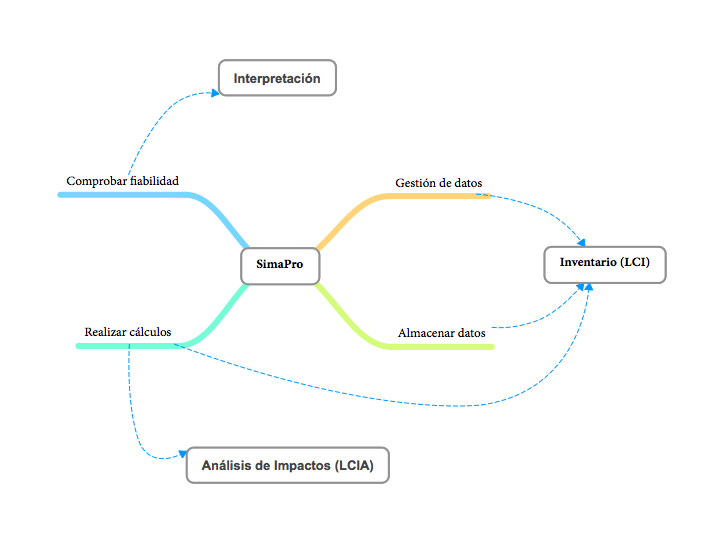
\includegraphics[width=15cm]{simapro.png}
\caption{Estructura de SimaPro.}
\label{fig:simapro}
\end{figure}

Entre sus principales cualidades destacan:

\begin{itemize}
  \item Diseño de productos.
  \item Desarrollo de indicadores clave.
  \item Cálculo de la huella de carbono de muchos tipos de productos y sistemas.
  \item Determinar el impacto medioambiental de productos o servicios con precisión estadística mediante el método de análisis Monte Carlo.
  \item Incluye Declaraciones Medioambientales de Productos e Informes Medioambientales GRI (Global Reporting Initiative).
  \item Utilización de bases de datos con inventarios.
  \item Asignación de múltiples procesos de salida.
  \item Análisis de Punto Débil, que permite identifica los puntos sensibles en el ciclo de vida utilizando un árbol de procesos.
  \item Análisis de tratamientos de residuos y escenarios de reciclado.
\end{itemize}

Esta herramienta cuenta con una interfaz de usuario intuitiva con un explorador de guía a través del Análisis de Ciclo de Vida del producto o servicio siguiendo los principios de las normas ISO 14040 y 14044. Además incorpora un modelado utilizando un asistente paso a paso.

La mayor ventaja de esta herramienta es la utilización de bases de datos con los inventarios de miles de procesos y métodos más importante de análisis de impacto.

\subsubsection{Bases de datos en SimaPro}
SimaPro incluye varias bases de datos de inventarios con miles de procesos, además de los métodos de análisis de impacto más importantes. De esta forma, no es necesario recolectar datos de procesos individuales y poder centrarse en los asuntos más importantes del estudio.

\begin{figure}[!htb]
\centering
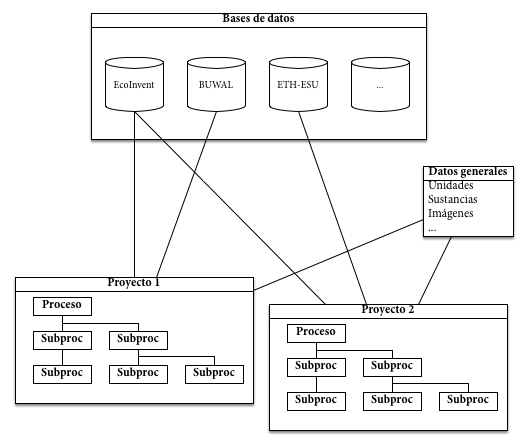
\includegraphics[width=15cm]{bbddsimapro.png}
\caption{Estructura de una base de datos de SimaPro.}
\label{fig:bbddsimapro}
\end{figure}

La calidad de los datos que aparecen en el Inventario de Ciclo de Vida (ICV) implica que el estudio sea relevante o no. \textit{ecoinvent} implementa en una única base de datos miles de conjuntos de datos de ICVs —agricultura, energía, transporte, combustibles, biomateriales, químicos, materiales de construcción, materiales de empaquetamiento, metales elementales y preciosos, procesado de metales, informática y electrónica, tratamiento de residuos— basados en información industrial recopilada por grupos de investigación y consultores reconocidos internacionalmente \cite{website:ecoinvent}.

\begin{figure}[!htb]
\centering
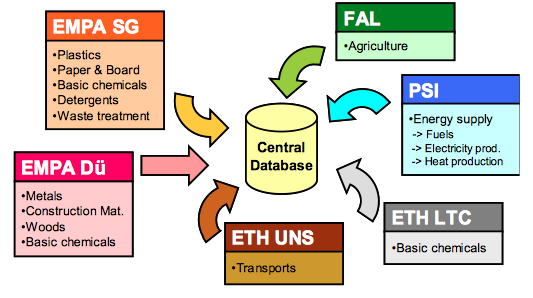
\includegraphics[width=13cm]{bbddecoinvent.png}
\caption[Estructura de la base de datos de \textit{ecoinvent}.]{Estructura de la base de datos de \textit{ecoinvent}. Fuente: \protect\cite{mgoedkoop2}.}
\label{fig:bbddecoinvent}
\end{figure}

De esta forma, la metodología de uso de SimaPro consiste en utilizar \textit{ecoinvent} como soporte para aquellos materiales y procesos de nuestro sistema que sean similares con los de la base de datos. En caso de que no se adapten a la entrada de la base de datos será necesario modelar una nueva entrada equivalente, pudiendo usar otras entradas de la base de \textit{ecoinvent}.

La librería \textit{ecoinvent}:
\begin{itemize}
  \item Incorpora más de 4000 procesos:
  \begin{itemize}
    \item Bienes de producción y calidades.
    \item Para algunos procesos añade diferencias regionales (Suiza y Unión Europea).
    \item Mix eléctrico y procesos agrícolas de Estados Unidos y Asia.
  \end{itemize}
  \item Incertidumbre en los datos.
  \item Ilustraciones de la mayoría de los procesos.
  \item Documentación extensa y consistente de los procesos.
  \item Actualizaciones frecuentes y periódicas.
  \item Incluye versiones de los procesos como Unidad (Proceso 1/U) —más detallado— o como Sistema (Proceso 1/S) —sin información de incertidumbre—.
\end{itemize}

\section{Metodología para Evaluación del Impacto del Ciclo de Vida}
\subsection{ReCiPe}\label{sec:recipe}

El desarrollo de ReCiPe se debió en principio a integrar la metodología orientada al problema de \textit{CML-IA} y la metodología orientada al daño de \textit{Ecoindicator 99}. De esta manera, ReCiPe se convirtió en el sucesor de ambos métodos \cite{mgoedkoop3}.

La metodología orientada al problema de \textit{CML-IA} define las categorías de impacto en el punto medio. La incertidumbre de los resultado en este punto es relativamente baja. El inconveniente de este sistema es la ambigüedad de las conclusiones al haber demasiadas categorías de impacto.

La metogología orientada al daño de \textit{Ecoindicator 99} aborda sólo tres categorías de impacto, lo que hacer más fácil obtener conclusiones. Sin embargo, la incertidumbre de los resultados es más alta que con la otra metodología.

ReCiPe implemente ambas estrategias incluyendo las categorías de impacto tanto a punto medio como a punto final. A los factores de caracterización a punto medio se les aplica un factor de daño para obtener los valores de caracterización de punto final. ReCiPe comprende dos conjuntos de categorías de impacto (ver figura ref{recipecategoriasimpacto}):
\begin{itemize}
\item Punto medio: 18 categorías de impacto.
\item Punto final: 3 categorías de impacto.
\end{itemize}

\begin{figure}[!htb]
\centering
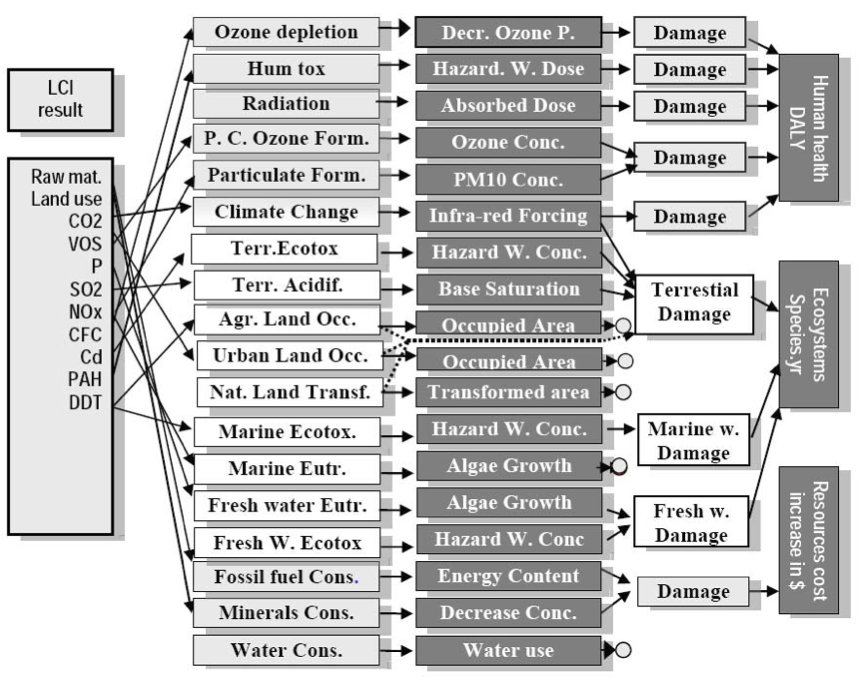
\includegraphics[width=12cm]{recipecategoriasimpacto.png}
\caption[Categorías de impacto aplicadas por ReCiPe.]{Categorías de impacto aplicadas por ReCiPe. Fuente: \protect\cite{mgoedkoop3}.}
\label{fig:recipecategoriasimpacto}
\end{figure}

\subsection{Demanda de Energía Acumulada}

\subsection{IPCC 2007}


